\fancychapter{Background}

In this Section we will start by generally describing what Clustering is and how it works. We will then outline how Self-Organizing maps~\cite{Kohonen1990} function, which is the Document Clustering algorithm used on this project.

\section{Document Clustering}
\label{sec:clustering}
Document clustering is an optimal division of documents into categories without prior knowledge of the data that is being organized, based only on the similarity between them. Due to the fact that no prior knowledge of the data has to be known, Document Clustering is labeled as Unsupervised Machine Learning~\cite{hinton1999unsupervised}.

~\citet{Liu2012b} asserted that Document Clustering can be used in a variety of Computer Science fields, such as:
\begin{itemize}
  \item Natural Language Preprocessing.
  \item Automatic Summarization.
  \item User preference mining.
  \item Improving text classification results.
\end{itemize}

There are two main types of Document Clustering: Hard Clustering and Soft Clustering. In Hard Clustering one document can only belong to one cluster, while in Soft Clustering one document can belong to multiple clusters. 

%REMOVEDBYPAVEL
%In regard to document categorization~\citet{Springorum1998} performed clustering with SOMs~\citep{Kohonen1990} while identifying polysemous German Propositions. They used regular SOMs to create multiple clusters and used Centroid-Based or Preposition-based softening to create Soft Clusters from the Hard Clusters.

The clustering process usually works as described in Figure~\ref{fig:1_Text_Clustering_Main_Framwork}
\begin{figure}
  \begin{center}
    \includegraphics[width=12cm]{images/1_Text_Clustering_Main_Framwork.png}
  \end{center}
  \caption{ Text clustering main framework~\cite{Dozono2012} }
  \label{fig:1_Text_Clustering_Main_Framwork}
\end{figure}
In the first, step a data set must be provided with the documents, to be clustered. The second step is where non relevant words are removed from the documents, to improve clustering quality~\cite{Kang2003}. 
%REMOVEDBYPAVEL
%Another way to extract keywords is to differentiate text features by analyzing the document corpora. For example if the dataset is composed from HTML or XML documents it is possible to identify more relevant features due to the characteristics of the document syntaxe.
The third step is characterized by converting the keywords of each document into vectors. The most common model used for this task is \ac{VSM}. In \ac{VSM}, each vector dimension represents one detected keyword and each document is represented by the vector of keywords in the feature space. This process is ilustrated in Figure~\ref{fig:2_svm} and works in the following way:
\begin{itemize}
  \item First step: string tokenization, and token selection. In this case stop words and repeated words will be removed.
  \item Second step: string to \ac{VSM} convertion. Each diferent word will correspond to a position in the array, and its value will correspond to the number of ocurrences. 
\end{itemize}

\begin{figure}
  \begin{center}
    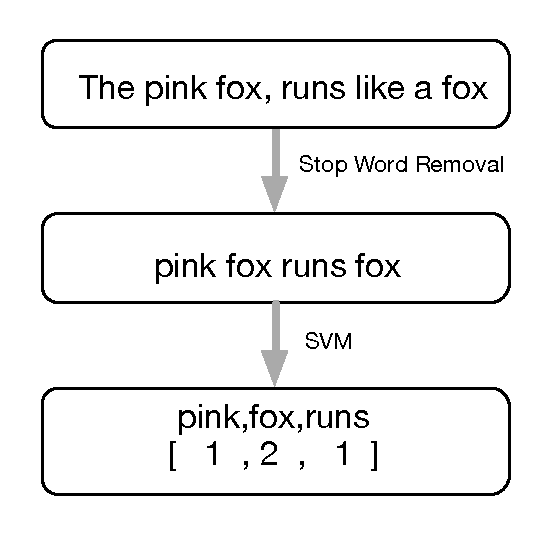
\includegraphics[width=5cm]{images/2_svm.eps}
  \end{center}
  \caption{ Text tokenization and transformation to Vector Space Model. }
  \label{fig:2_svm}
\end{figure}

There are many clustering algorithms. In the following section we will describe the particullar case of the \ac{SOM}, the solution used in our work.

\section{The Self-Organizing Map} 
\label{sec:the_self_organizing_map}

\ac{SOM} are a two layer, recurrent \ac{ANN} that has the desired property of topology preservation, thus mimiking the way the cortex of highly developed animals brains work. \ac{SOM} allow cluster visualization of multi-dimensional data, similar to methods such as \ac{MDS}~\cite{KruskalWish1978} and \ac{PCA}~\cite{Hotelling_1933} .  

As \citet{Bacao2005} describes, the basic idea behind SOM is to map the data patterns into an n-dimensional grid of neurons, or units. That grid is also know as the output space, as opposed to the initial space, called input space, where the input patterns reside. Both spaces can be seen in Figure~\ref{fig:5_neighbours_converge}.

SOMs work similarly to the way that is thought that the human brain works. By having a set of neurons that, through learning experience, specialize in the identification of certain types of patterns. These neurons are responsible for categorizing the input patterns for which they are responsible to identify. Nearby neurons will be organized by similarity, which will cause similar patterns to activate similar areas of the \ac{SOM}.
With this topology preserving mapping, the SOM organizes information spatially, where similar concepts are mapped to adjacent areas. The topology is preserved in a sense that, as far as possible, neighborhoods are preserved throughout the mapping process.
Output neurons are displayed in an N dimensional grid, generally rectangular, but other structures are possible, such as hexagonal or octagonal.  The grid of neurons in the output space, can be divided in neighborhoods, where neurons responsible for the same kind of input reside.
In SOM, neurons will have the same amount of coefficients as the input patterns and can be represented as vectors.

Before describing the algorithm it is important to define two key aspects of the SOM, the learning rate and the quantization error. The learning rate is a function that will be decreased to converge to zero. It will be applied to winning neurons and their neighbors in order for them to move toward the corresponding input pattern in progressively smaller steps. Quantization Error is the distance between a given input pattern and the associated winning neuron, it describes how well neurons represent the input pattern. The radius of the neighborhood around the winner neuron is also particularly relevant to the topology of the SOM, deeply affecting the unfolding of the output space as stated by \citep{Bacao2005}.
\par

\input{./algorithms/som.tex}

\begin{figure}[h]
  \begin{algorithm}[H]
    \label{alg:umatrix}
    \DontPrintSemicolon
    \KwData{$W = \{  \overrightarrow{w_{0,0}}$,\dots,$\overrightarrow{w_{n,n}}$ \} are the trained neurons 

            $D_{i,j}$ be the input patterns represented with neuron $w_{i,j}$

            $U$ is an empty matrix with size $2n-1.2n-1$
  }
    \KwResult{U-Matrix}
    \tcc{Initialize $U$ by adding the trained neurons}
    \For{ $w_{ij} = \overrightarrow{w_{00}}$ to $\overrightarrow{w_{n,n}}$ }{
      $U_{i*2, j*2} \leftarrow w_{i,j}$
    }
    \tcc{Calculate the distance between every adjacent neurons, and apply it to the square between them}
    \For{ $i=0$ to $U_{max}$}{
           
      \For{  $j=0$ to $U_{max}$}{
        
        \If{$l+1<m || j+1<m$}{
          $U_{i+1, j} = \| u_{i,j} - u_{i+2,j} \| $
          $U_{i, j+1} = \| u_{i,j} - u_{i,j+2} \| $
          $U_{i+1, j+1} = \frac{\| u_{i,j} - u_{i+2,j+2} \| + \|u_{i+2,j} - u_{i,j+2} \| }{2}$

        }
        $ j \leftarrow j + 1 $
      }
      $ i \leftarrow i + 1 $
    }
    \tcc{Substitute the neurons for an average of surrounding distances}
    \For{ $i=0$ to $U_{max}$}{
      \For{  $j=0$ to $U_{max}$}{
        $ u_{ij} = avg( Adj[u_{ij}] )$

        $ j \leftarrow j + 1 $
      }
      $ i \leftarrow i + 1 $
    }
    \tcc{convert the distances to color}
    $WHITE = 255$

    $BLACK = 0$

    $ u_{max} \leftarrow max(U) $

    $ u_{min} \leftarrow min(U) $

    \For{ $u_{ij} = u_{00}$ to $u_{n,n}$ }{
      $U_{i, j} \leftarrow (1 - \frac{ u_{i,j} - u_{min}  }{u_{max}-u_{min}})* WHITE$
    }
    \caption{U-Matrix }
  \end{algorithm}
\end{figure}


\begin{figure}
  \begin{center}
    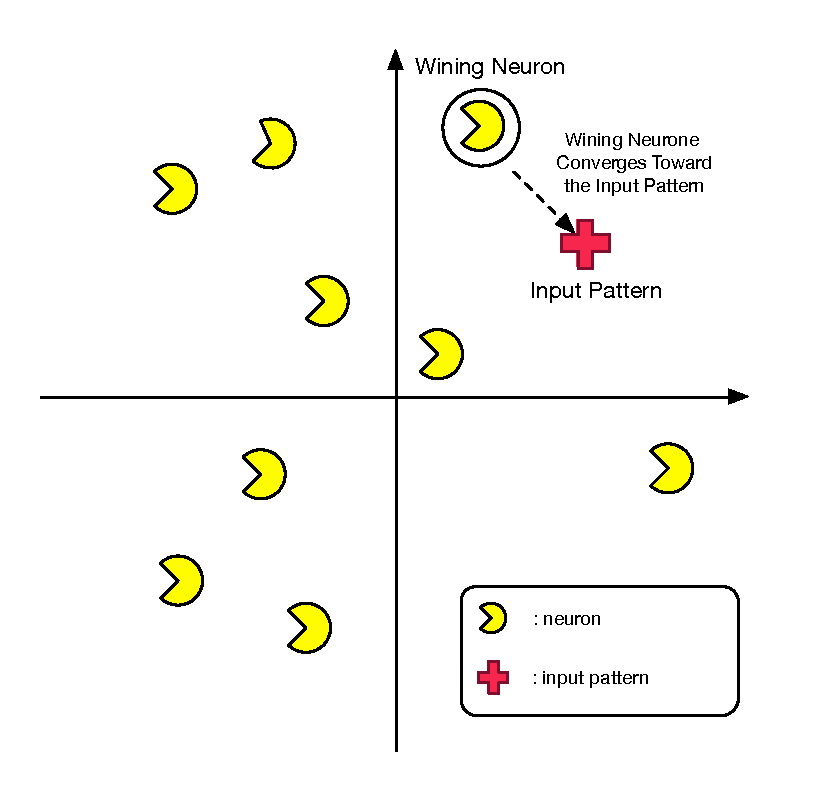
\includegraphics[width=5cm]{images/4_wining_neuron_converge.eps}
  \end{center}
  \caption{ Winning neuron converging at learning rate }
  \label{fig:4_wining_neuron_converge}
\end{figure}

\begin{figure}
  \begin{center}
    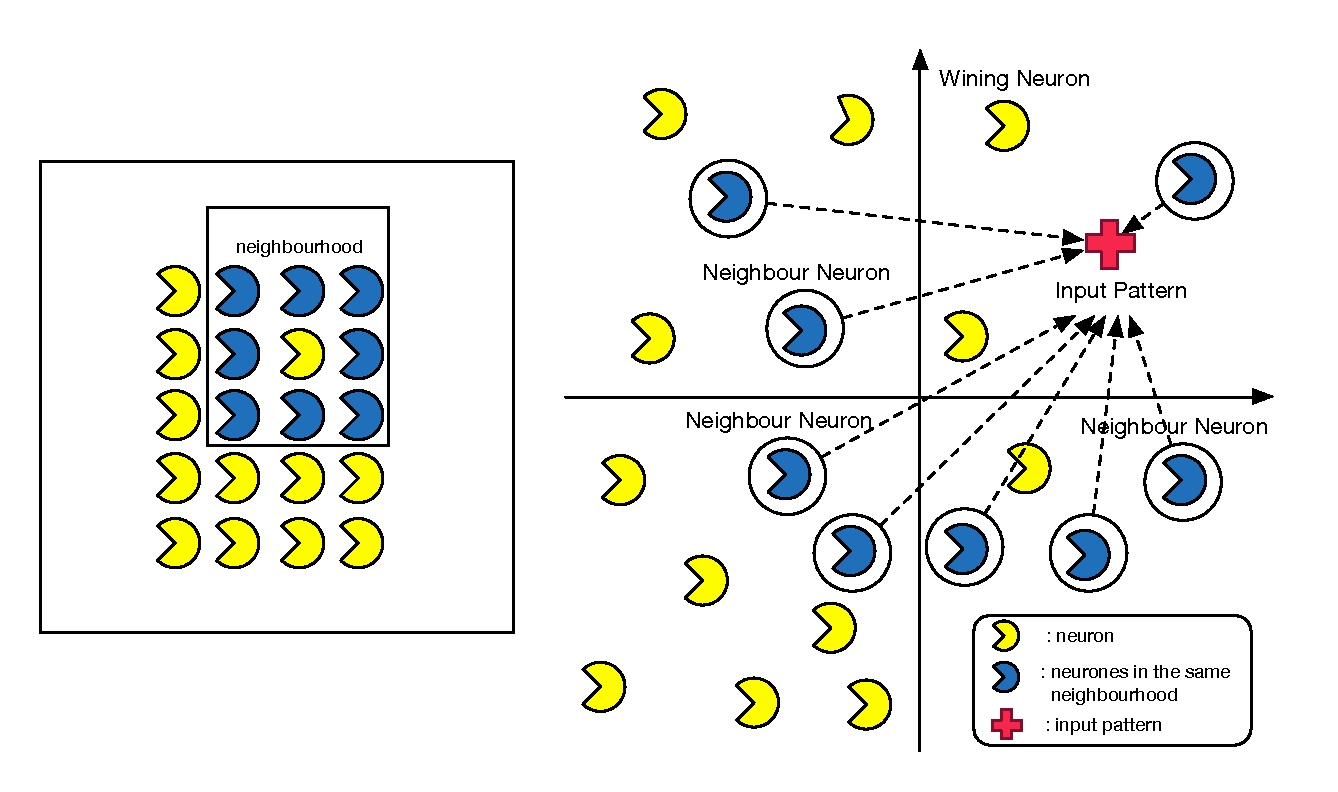
\includegraphics[width=12cm]{images/5_neighbours_converge.eps}
  \end{center}
  \caption{ On the left the output space neighborhood, on the right the neighbors of the winning neuron converging in the direction of the input pattern }
  \label{fig:5_neighbours_converge}
\end{figure}

The prediction phase can start after the model is learned. On the prediction phase new input patterns can be quickly assigned to the \ac{SOM}, without need to apply the learning rate to the winning neuron and his neighbors. Due to the fact that the input pattern will be assigned to the cluster that the nearest neuron is mapping. Thus it very easy and fast to classify new data now.

%\begin{equation}
  \label{eq:exp_decay}
  \frac{dN}{dT}=-\lambda N
\end{equation} 



In order to visually interpret the result of the \ac{SOM}, \ac{U-Matrix} method may be used~\citep{Bacao2005}. The \ac{U-Matrix} is a representation of the \ac{SOM} in which distances, in the input space between neurons is represented using a gray scale.

The advantages of using \ac{SOM} is data noise immunity, easy to visualize the data, and parallel processing~\cite{Liu2012b}.
 
